\newcommand{\descriereIdempotenta}{Termenul \textit{"idempotență"} este folosit pentru a evidenția faptul că o parte dintre operațiile efectuate de către mecanismul automatizat de generare a infrastructurii vor avea același rezultat dacă vor fi apelate de mai multe ori. Din motive de securitate, unele operații vor fi definite explicit ca nefiind idempotente (e.g. generarea de chei de acces pentru API-ul 'Surf', generarea adresei de acces a API-ului (nu va fi suprascrisă în API-ul existent)) }

Procesul de generare a infrastructurii (engl. 'deployment') constă în crearea resurselor și pornirea sistemelor necesare pentru ca web-crawler-ul 'Surf' sa funcționeze. Mecanismul de generare a resurselor execută următorii pași:

\begin{itemize}

	\item{Crearea entităților necesare în AWS (e.g. funcții Lambda, roluri IAM, API-ul APIGateway etc.);}
	
	\item{Stabilirea relațiilor între resurse și injectarea dependențelor (e.g. unei rute a API-ului trebuie să îi fie asociat un rol IAM care să îi permită invocarea unei funcții Lambda);}
	
	\item{Generarea SDK-ului Javascript necesar pentru a putea invoca API-ul 'Surf' din cadrul clientului web;}
	
	\item{Generarea unui fișier de configurare injectabil în clientul web 'Surf' pentru a stabili parametrii interacțiunii între client și cloud-ul AWS (e.g. regiunea AWS în care s-a generat infrastructura, metadate legate de rolurile utilizatorilor, cheia generată pentru a restricționa accesul asupra API-ului etc.).}

  \item{Generarea unui fișier de configurare injectabil în pachetul ce conține codul funcțiilor Lambda, în vederea efectuării setărilor legate de mecanismul asincron de notificare, numele bucket-urilor S3 create etc.}
\end{itemize}

\noindent
Efortul necesar pentru generarea infrastructurii este mare, datorită complexității inerente a proiectului. Efectuarea manuală a pașilor în interfața web AWS (engl. "AWS Web Console") necesită foarte mult timp și este predispusă la erori. De asemenea, asigurarea disponibilității crawler-ului în mai multe regiuni globale AWS, sau pe mai multe conturi AWS, ar necesita repetarea identică a pașilor enumerați mai sus, pentru fiecare astfel de regiune sau cont. De aceea, crawler-ul web 'Surf' pune la dispoziție o modalitate automatizată de deployment, configurabilă, testabilă și reutilizabilă, asigurând idempotență\footnote{\descriereIdempotenta} la nivelul efectuării operațiilor în cadrul AWS.
\\

\noindent
Mecanismul automatizat de generare a infrastructurii AWS reprezintă un program care primește, ca date de intrare, un fisier de configurare în format JSON, generează resursele AWS și oferă clientului web, ca date de ieșire, prin injectarea dependențelor, informații și mecanisme pentru utilizarea infrastructurii create. Cerințele pentru execuția cu success a deployment-ului, precum și validitatea resurselor generate, reprezintă existența credențialelor AWS necesare pentru pașii de deployment (e.g. IAM 'administrator-access') și generarea pachetului în format \emph{.jar}, care să conțină codul funcțiilor Lambda care se doresc a fi încărcate în AWS. Mai jos, se poate observa un exemplu de fișier de configurare pentru generatorul de resurse AWS 'Surf':

\begin{figure}[ht]
\begin{minted}[fontsize=\footnotesize]{json}
{
  "awsAccountId": "011759591962",
  "awsAccessKey": "#######", // Ascuns intenționat
  "awsClientRegion": "eu-west-1",
  "lambdaCodePath": "../lambda/target/surf-lambda-backend-1.0-SNAPSHOT.jar",
  "lambdaRuntime": "java8",
  "apiGatewayEndpoint": "apigateway.amazonaws.com",
  "apiStageName": "v1",
  "apiStageMetricsEnabled": true,
  "apiStageThrottlingRateLimit": "5",
  "apiStageThrottlingBurstLimit": "20",
  "apiLoggingLevel": "INFO",
  "apiGeneratedSdkType": "javascript",
  "apiGeneratedSdkOutputPath": "../../frontend/generated/sdks/",
  "apiGeneratedSdkFolderName": "api-gateway-js-sdk",
  "clientConfigFilePath": "../../frontend/generated/config/aws-config.json",
  "lambdaConfigFilePath": "../lambda/generated/config/lambda-config.json",
  "dynamoDBWorkflowsTableReadCapacityUnits": "2",
  "dynamoDBWorkflowsTableWriteCapacityUnits": "2"
}
\end{minted}
\begin{center}
	\caption{Fișier parțial de configurare (intrare) pentru generatorul de resurse}\par\medskip
	\vspace*{-20pt}
\end{center}
\end{figure}

\noindent
Pentru a asigura conexiunea clientului web cu infrastructura creată, generatorul de resurse AWS injectează un fișier de configurare în clientul web, într-un director special destinat acestui sens. Politicile de securitate implementate în generatorul de resurse nu vor permite suprascrierea fișierului/directorului din clientul web în cazul în care acesta există deja, pentru a evita pierderea datelor. Un astfel de fișier de configurare este cel prezentat în \textit{Figura 5}:
\\

\begin{figure}[ht]
\begin{minted}[fontsize=\footnotesize]{json}
{
  "awsClientRegion": "eu-west-1",
  "awsAccessKey": "#######", // Ascuns intenționat
  "facebookWebIdentityBasicRoleArn": "arn:aws:iam::011759591962:role/fb-role",
  "apiKey": "#######" // Ascuns intenționat
}
\end{minted}
\begin{center}
	\caption{Fișier folosit pentru configurarea clientului}\par\medskip
	
\end{center}
\end{figure}

\noindent
Diagrama din \textit{Figura 6} prezintă procesul de construire a infrastructurii, ordonând temporal pașii necesari pentru crearea și configurarea crawler-ului. Înainte de începerea deployment-ului resurselor AWS, se generează o arhivă ce conține codul sursă al funcțiilor Lambda. Procesul începe cu citirea fișierului de configurare și se încheie cu generarea API-ului prin care utilizatorii vor putea accesa serviciul web. Acolo unde este necesar, se specifică interdependențele între sisteme. De exemplu, este necesar ca mai întâi să fie create funcțiile Lambda, înainte ca acestea să fie înregistrate în cadrul mecanismului de notificare asincronă oferit de SNS (de aici și numarul 4 asociat generării funcțiilor Lambda, reprezentând o prioritate mai mare decât numarul 5 asociat serviciului SNS). După finalizarea procesului de generare a infrastructurii, pașii 1 si 4 se vor rula încă odată, în contextul execuției precedente (i.e. având la dispoziție toate referințele către resursele create), pentru a actualiza codul funcțiilor Lambda în vederea accesării resurselor menționate.

\begin{figure}[ht]
\begin{center}
	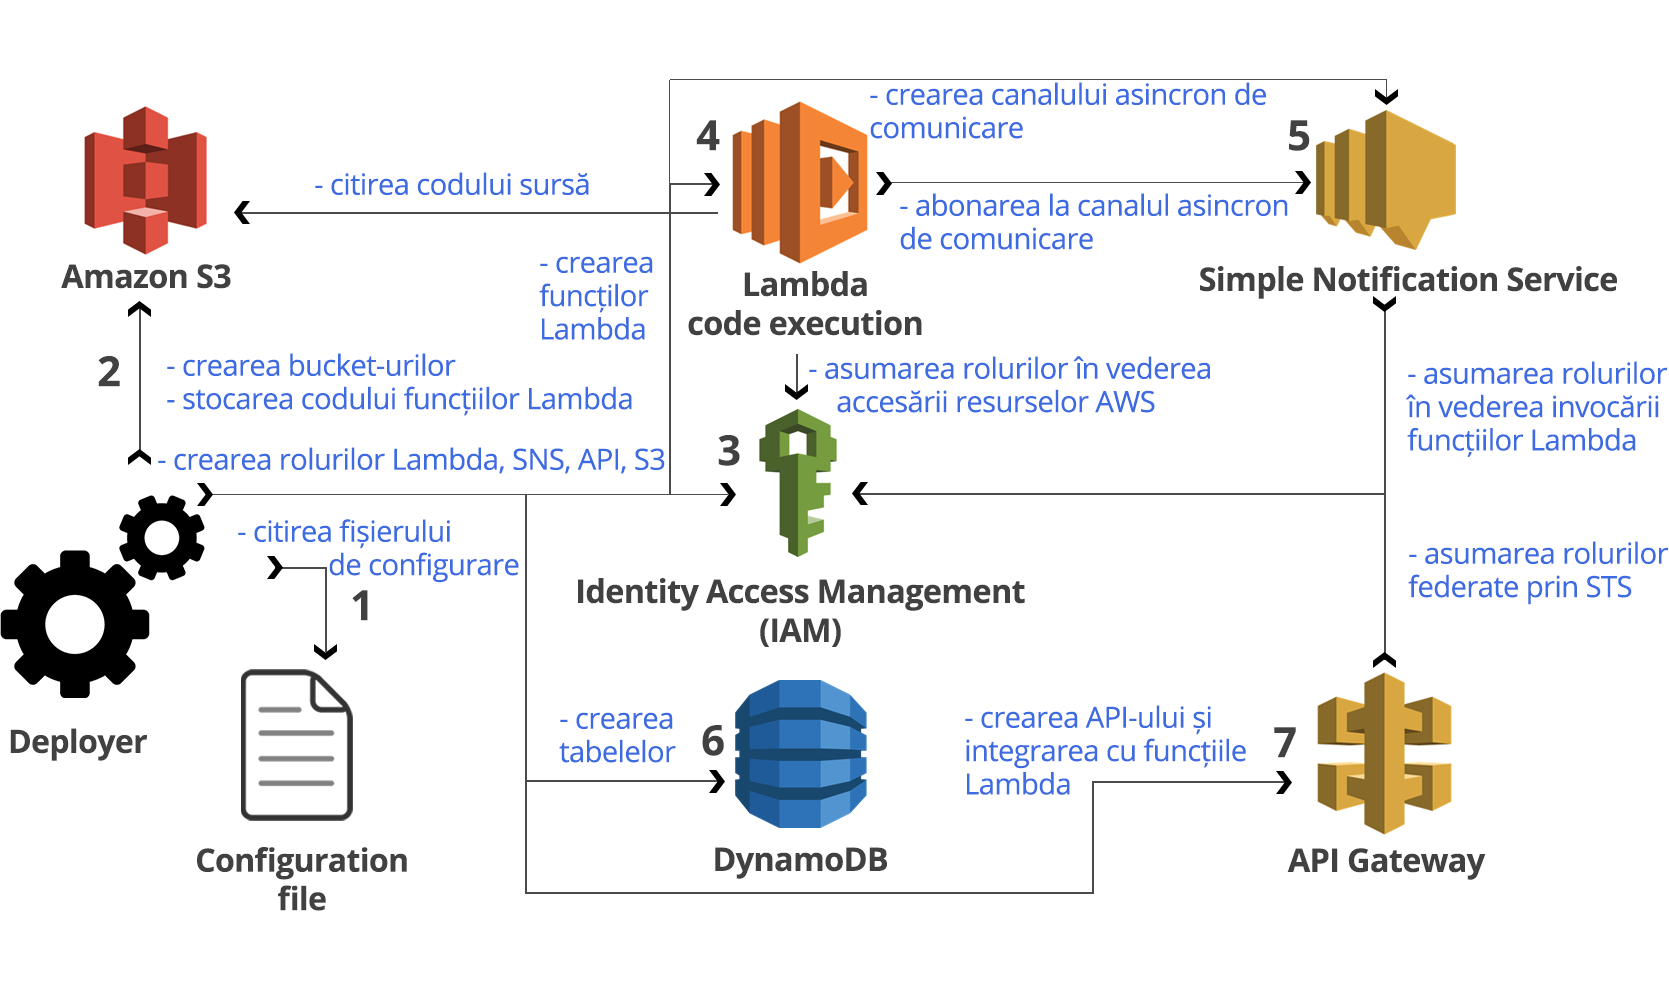
\includegraphics[keepaspectratio, width=1.0\textwidth]{generare-infrastructura.png}
	\caption{Generarea infrastructurii \cite{diagram-icons-sources, aws-icons-source}}\par\medskip 

\end{center}
\end{figure}

 